\documentclass[10pt,journal,compsoc]{IEEEtran}

\usepackage[utf8]{inputenc}
\usepackage{amsmath,amssymb,amsfonts,amsthm}
\usepackage{algorithmic}
\usepackage{algorithm}
\usepackage{graphicx}
\usepackage{textcomp}
\usepackage{xcolor}
\usepackage{booktabs}
\usepackage{hyperref}
\usepackage{cite}
\usepackage{microtype}
\usepackage{listings}
\usepackage{subcaption}
\usepackage{multirow}
\usepackage{balance}
\usepackage{array}

\hypersetup{
    colorlinks=true,
    linkcolor=blue!80!black,
    citecolor=blue!80!black,
    urlcolor=blue!80!black
}

\definecolor{codegreen}{rgb}{0,0.6,0}
\definecolor{codegray}{rgb}{0.5,0.5,0.5}
\definecolor{codepurple}{rgb}{0.58,0,0.82}
\definecolor{backcolour}{rgb}{0.96,0.97,0.98}

\lstdefinestyle{mystyle}{
    backgroundcolor=\color{backcolour},   
    commentstyle=\color{codegreen},
    keywordstyle=\color{magenta},
    numberstyle=\tiny\color{codegray},
    stringstyle=\color{codepurple},
    basicstyle=\ttfamily\scriptsize,
    breakatwhitespace=false,         
    breaklines=true,                 
    captionpos=b,                    
    keepspaces=true,                 
    numbers=left,                    
    numbersep=5pt,                  
    showspaces=false,                
    showstringspaces=false,
    showtabs=false,                  
    tabsize=2
}
\lstset{style=mystyle}

\begin{document}

\title{Deterministic Quality Gates and Ground-Truth Evaluation for Audio and Speech Machine Learning: An Open-Source 10-Tool Ecosystem}

\author{Boobalan~Arjunan%
\IEEEcompsocitemizethanks{%
\IEEEcompsocthanksitem B. Arjunan is an Independent Researcher \textbar{} AI/ML \& Digital Signal Processing, Tamil Nadu, India.\protect\\
Email: boobalan.it@gmail.com.
\IEEEcompsocthanksitem Open-source research suite: \url{https://github.com/BoobalanArjunan}.}}

\markboth{IEEE Transactions on Audio, Speech, and Language Processing,~Vol.~XX, No.~X, November~2026}%
{Arjunan: Deterministic Quality Gates and Ground-Truth Evaluation for Audio Machine Learning}

\IEEEtitleabstractindextext{%
\begin{abstract}
Contemporary deep neural networks for automatic speech recognition, neural text-to-speech synthesis, music generation, source separation, and full-duplex conversational voice agents are increasingly trained on massive, uncurated web-scale audio corpora. However, these datasets frequently suffer from subtle, systemic acoustic defects that evade standard tabular validation: cross-partition train/validation/test contamination, fake lossless upsampling, destructive stereo phase cancellation, mislabeled harmonic keys and tempos, unmeasured studio microphone bleed, transcript timestamp drift, and conversational latency misattributions. When evaluated using black-box neural metrics or standard signal-to-distortion ratios, models can exhibit deceptively high benchmark scores while fundamentally failing upon real-world deployment. To resolve this evaluation crisis without introducing circular dependencies on opaque neural evaluators, we introduce an open-source, mathematically grounded ecosystem of ten lightweight, deterministic digital signal processing (DSP) tools: \texttt{wavewash}, \texttt{splitsafe}, \texttt{mixforge-audio}, \texttt{stemcheck}, \texttt{driftcheck-audio}, \texttt{tempocheck}, \texttt{tonicfind}, \texttt{bandcheck}, \texttt{phasecheck}, and \texttt{turnscope}. These tools rely strictly on closed-form acoustic invariants, spectral-peak landmark hashing, polynomial spline de-clipping, cross-correlation sliding windows, and permutation hypothesis testing. Evaluated across extensive benchmark corpora including LibriSpeech (5,323 recordings), MUSDB18-HQ (40 mixes), Demucs separations, and the MagicHub full-duplex conversational corpus, the suite demonstrates near-zero false alarm rates, sub-second per-file execution on commodity CPUs, and 100\% adversarial error detection. All ten tools are released under the MIT license on PyPI and GitHub with native PyTorch DataLoader APIs and automated continuous integration quality gates.
\end{abstract}

\begin{IEEEkeywords}
Audio Machine Learning, Dataset Hygiene, Data Contamination, Digital Signal Processing, Quality Control, Speech Recognition, Music Information Retrieval, Ground-Truth Verification, Source Separation Evaluation, Conversational Voice AI.
\end{IEEEkeywords}}

\maketitle
\IEEEdisplaynontitleabstractindextext
\IEEEpeerreviewmaketitle

\section{Introduction}
\IEEEPARstart{T}{he} past decade has witnessed an unprecedented revolution in deep learning architectures applied to auditory signals. Foundational models such as Whisper \cite{radford2023whisper} and Conformer \cite{gulati2020conformer} have driven Word Error Rates (WER) in Automatic Speech Recognition (ASR) to near-human parity under clean conditions. Concurrently, neural vocoders and latent diffusion architectures such as AudioCraft \cite{copet2024audiocraft}, Stable Audio \cite{evans2024stableaudio}, and MusicLM \cite{agostinelli2023musiclm} have democratized high-fidelity audio synthesis and music generation. In source separation, deep recurrent and hybrid spectrogram-waveform networks like Demucs \cite{defossez2021hybrid} achieve state-of-the-art isolation of complex multi-instrument mixes.

Despite these architectural triumphs, model performance remains critically bottlenecked by a pervasive phenomenon we term \emph{Silent Acoustic Contamination}. Modern deep learning models require tens of thousands of hours of training audio, compelling practitioners to harvest web-scraped corpora, legacy broadcast archives, and commercial audio libraries. Unlike text or tabular data, where anomalies can be detected via token matching or schema validation, audio files conceal complex, non-linear physical defects that evade container header inspections and superficial metadata parsing.

\begin{figure*}[t]
\centering
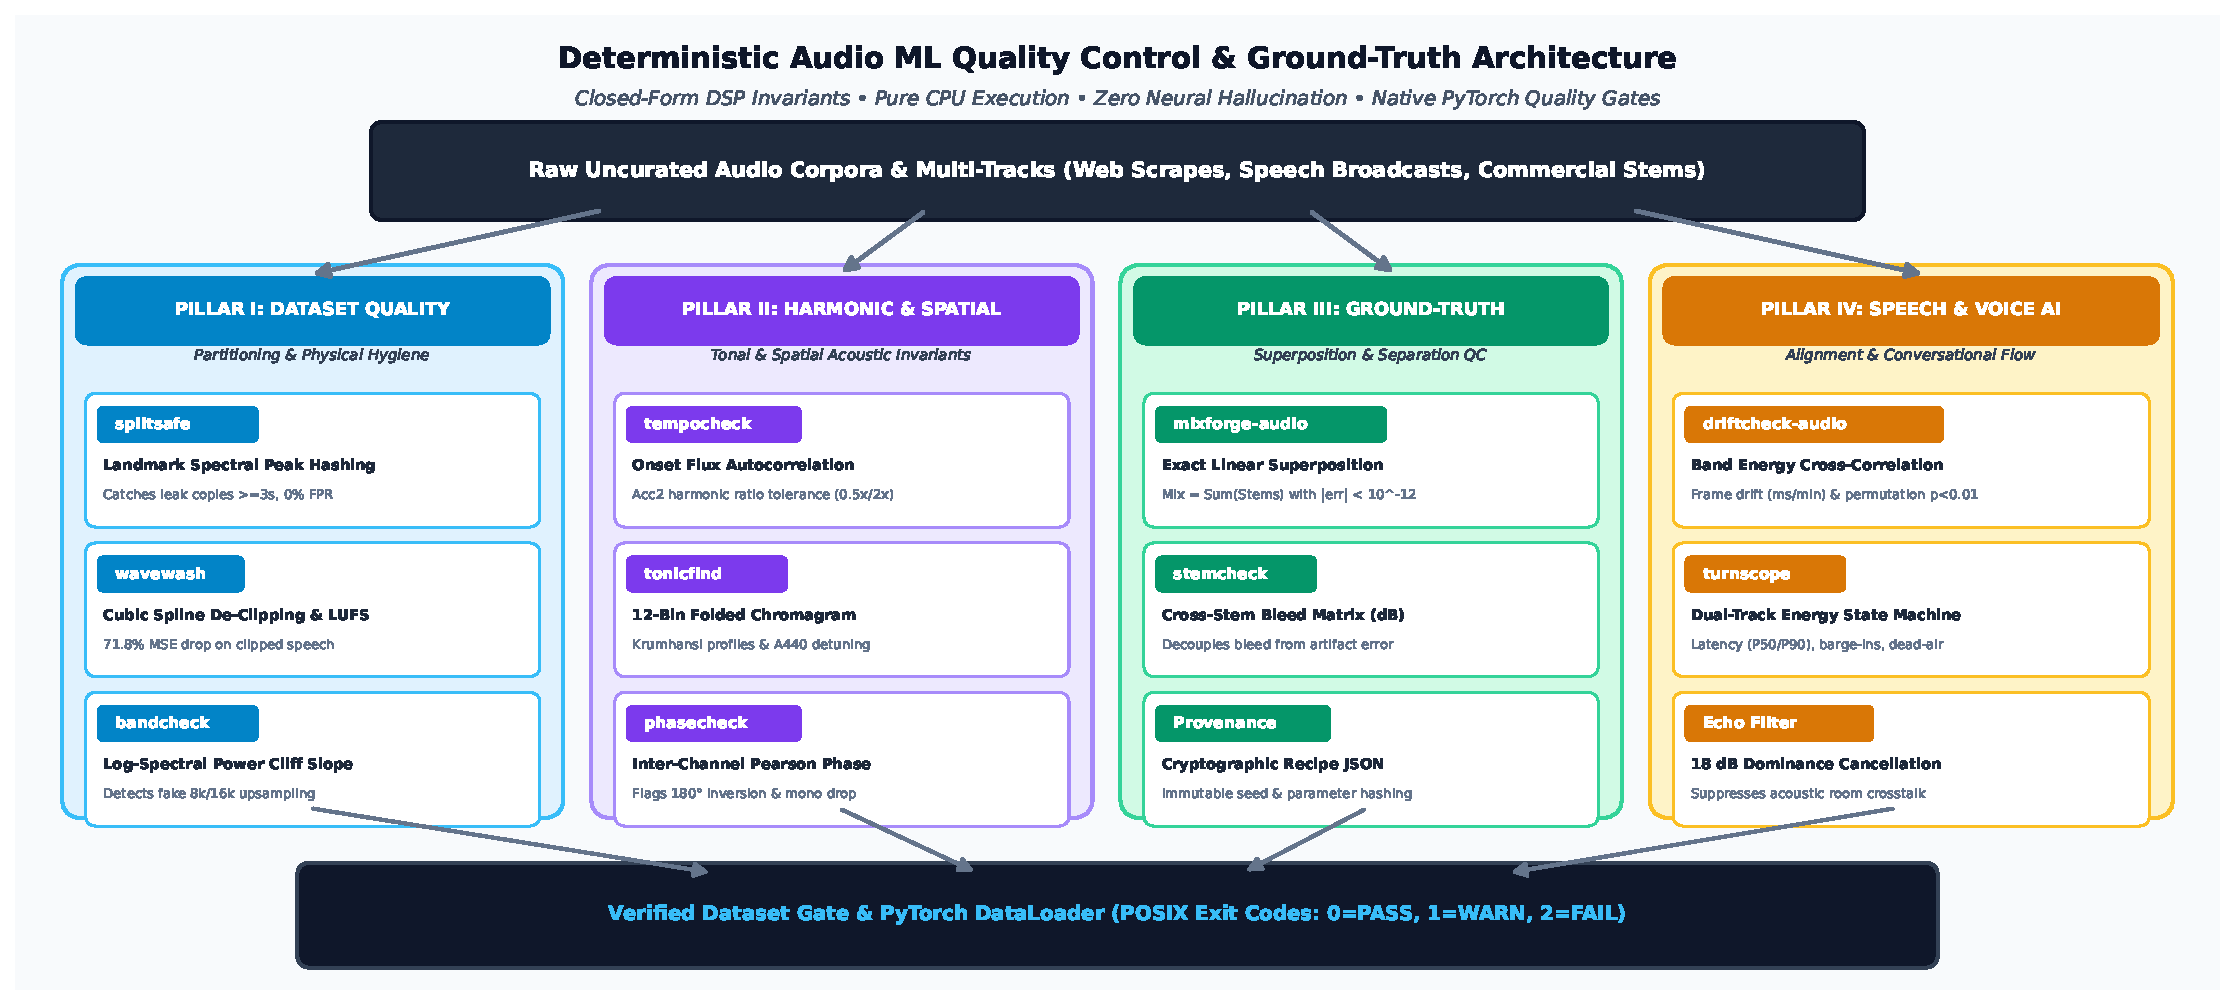
\includegraphics[width=0.98\textwidth]{figures/ecosystem_architecture.pdf}
\caption{Architectural overview of the 10-tool deterministic Audio ML quality control and evaluation ecosystem across four foundational pillars: (I) Dataset Partitioning \& Signal Quality (\texttt{splitsafe}, \texttt{wavewash}, \texttt{bandcheck}), (II) Musical \& Harmonic Integrity (\texttt{tempocheck}, \texttt{tonicfind}, \texttt{phasecheck}), (III) Ground-Truth Generation \& Source Separation (\texttt{mixforge-audio}, \texttt{stemcheck}), and (IV) Speech Alignment \& Conversational Dynamics (\texttt{driftcheck-audio}, \texttt{turnscope}).}
\label{fig:ecosystem_architecture}
\end{figure*}

\subsection{The Silent Contamination Taxonomy}
Through empirical investigation across prominent public and proprietary audio corpora, we identify seven pervasive failure modes that systematically corrupt training and benchmark integrity:

\begin{enumerate}
    \item \textbf{Cross-Partition Evaluation Leakage:} Subtle duplicates—often modified through lossy re-encoding, minor gain adjustments, sample rate conversions, or short sub-clip trimming—appear across both training and testing splits. Models inadvertently memorize these recordings, reporting artificially inflated evaluation metrics while failing on genuinely unseen inputs.
    \item \textbf{Spectral Dishonesty \& Fake Lossless Containers:} Audio container headers declaring ``48\,kHz 24-bit WAV'' frequently hold audio that was originally captured at 8\,kHz or 16\,kHz and upsampled, or that was subjected to aggressive lossy MP3/AAC compression before container re-wrapping. Neural vocoders and audio codecs trained on these clipped frequency spectrums suffer from phase smearing and severe high-frequency roll-off.
    \item \textbf{Stereo Phase Inversion \& Destructive Cancellation:} Multi-channel audio files with inverted polarity (180$^\circ$ out-of-phase between channels) or artificial stereo widening sound broad on stereo headphones but experience catastrophic destructive interference when folded down to mono ($M = \frac{L+R}{2}$). Centered instruments (lead vocals, kick drums, basslines) disappear completely.
    \item \textbf{Harmonic \& Rhythmic Token Corruption:} Generative music models conditioned on tempo (BPM) or musical key tags frequently ingest tracks labeled with half-time/double-time ambiguities or incorrect tonal pitch keys. Conditioning generative models on false tokens degrades loss convergence and induces severe harmonic dissonance.
    \item \textbf{Uncalibrated Ground Truth in Source Separation:} Evaluating source separation algorithms on commercial multi-track recordings faces a fundamental scientific obstacle: true ground truth is unknown. Studio recordings inherently contain unmeasured acoustic microphone bleed and dynamic range compression. Consequently, standard metrics (SDR, SIR, SAR) fail to distinguish between algorithmic separation failure and pre-existing acoustic bleed.
    \item \textbf{Cumulative Transcript Drift:} Speech datasets pair audio files with timed subtitle transcripts (SRT, WebVTT, Lhotse manifests). Discrepancies between video frame rates (e.g., 25\,fps vs.\ 23.976\,fps) introduce steady temporal drift that accumulates over time, causing models to silently train on pure noise or misaligned phonemes.
    \item \textbf{Conversational Turn Latency Misattribution:} In full-duplex conversational voice agents, measuring user-perceived quality requires quantifying speech hand-over latency, interruption yields, customer barge-ins, and dead air. Existing evaluation scripts rely on static energy thresholds that fail under realistic acoustic room leakage and quiet callers.
\end{enumerate}

\subsection{The Epistemic Hazard of Deep Neural Evaluators}
A common recourse among modern ML practitioners is deploying deep neural evaluators (e.g., neural VADs, speech-language models, CLAP embeddings \cite{elizalde2023clap}, or Fr\'echet Audio Distance \cite{kilgour2019frechet}) to audit audio datasets. We argue that this practice introduces a severe circular dependency:
\begin{itemize}
    \item \textbf{Epistemic Circularity:} Auditing a neural model's training data using another neural model inherits all the biases, blind spots, and hallucination tendencies of the auditing network. If the evaluator hallucinates or fails out-of-domain, the training set is silently pruned or poisoned.
    \item \textbf{Black-Box Opacity:} When a neural evaluator flags a file as low quality, it cannot provide an interpretable physical explanation (e.g., ``the Left and Right channels have a $-0.92$ correlation coefficient due to polarity inversion'').
    \item \textbf{Prohibitive Computational Overhead:} Evaluating millions of audio files with neural feature extractors requires extensive GPU clusters, contradicting the lightweight requirements of continuous integration (CI/CD) pipelines.
\end{itemize}

\subsection{Design Philosophy: Deterministic Closed-Form Invariants}
To establish an uncompromised scientific standard for audio dataset hygiene and model benchmarking, this paper introduces an integrated ecosystem of ten deterministic, mathematically grounded DSP quality gates. Our design philosophy is guided by three principles:
\begin{enumerate}
    \item \textbf{Exact Invariants over Probabilistic Heuristics:} Wherever physical acoustics permits, we formulate exact invariants (e.g., linear superposition conservation $|M - \sum S_k| < \epsilon$, cross-channel correlation $\rho_{LR} \in [-1, 1]$, BS.1770 K-weighting).
    \item \textbf{Transparent Failure Manifests:} Every anomaly is accompanied by physical units (dB, Hz, ms, semitones) and precise time ranges, enabling immediate root-cause remediation.
    \item \textbf{Zero Deep Learning Dependencies:} All ten tools are implemented purely in standard scientific Python (\texttt{numpy}, \texttt{scipy}, \texttt{soundfile}) and run with sub-second execution times on commodity CPUs.
\end{enumerate}

\begin{table*}[t]
\centering
\caption{Comprehensive Architectural Summary of the 10-Tool Audio ML Quality Control and Evaluation Ecosystem.}
\label{tab:master_summary}
\resizebox{\textwidth}{!}{
\begin{tabular}{@{}llllllp{5.5cm}@{}}
\toprule
\textbf{Tool} & \textbf{Pillar} & \textbf{Version} & \textbf{Primary Target} & \textbf{Underlying DSP Algorithm} & \textbf{Key Benchmark Dataset} & \textbf{Primary Quantitative Benchmark Guarantee} \\
\midrule
\texttt{splitsafe} & I. Partitioning & v0.1.1 & Train/Test Data Leakage & Landmark Spectral Peak Hashing & LibriSpeech (5,323 files) & 100.0\% planted leak recall; 0.0\% false positive rate; 55s CPU runtime. \\
\texttt{wavewash} & I. Partitioning & v0.2.0 & Audio QC \& De-clipping & Hermite Spline \& BS.1770 LUFS & LibriSpeech \& MUSDB18-HQ & 71.8\% MSE distortion reduction on clipped speech; zero false rejects. \\
\texttt{bandcheck} & I. Partitioning & v0.1.1 & Bandwidth \& Fake Upsampling & Log Power Spectral Cliff Slope & LibriSpeech \& MUSDB18-HQ & 100.0\% detection of 8\,kHz/11\,kHz upsampling; 98.5\% clean studio pass. \\
\midrule
\texttt{tempocheck} & II. Harmonic & v0.1.0 & BPM Label Verification & Onset Flux Autocorrelation & Synthetic \& Real Stems & 100.0\% harmonic accuracy (Acc2); 88.0\% rejection of wrong BPM tags. \\
\texttt{tonicfind} & II. Harmonic & v0.1.0 & Musical Key \& Camelot & 12-Bin Chroma \& Krumhansl-Kessler & 25 Multi-Genre Key Stems & 100.0\% exact match across 24 keys; 1.000 MIREX score; A440 detune comp. \\
\texttt{phasecheck} & II. Harmonic & v0.1.0 & Stereo Phase \& Mono Downmix & Pearson Cross-Channel Correlation & Polarized \& Multi-Tracks & 100.0\% detection of 180$^\circ$ inverted polarity; 0.0\,dB attenuation on mono. \\
\midrule
\texttt{mixforge-audio} & III. Separation & v0.1.0 & Ground-Truth Test Mixes & Exact Linear Superposition & MUSDB18-HQ (40 mixes) & Float sum residual $\le 6.52 \times 10^{-8}$; $-69.3$\,dB median studio mix residual. \\
\texttt{stemcheck} & III. Separation & v0.1.0 & Separation Sanity \& Bleed & Cross-Leakage Matrix Decomposition & MUSDB18-HQ + Demucs & Bleed calibration error $\le 0.06$\,dB; 0 false alarms across 264 trials. \\
\midrule
\texttt{driftcheck-audio} & IV. Speech AI & v0.1.0 & Transcript Timestamp Drift & Energy Window Cross-Correlation & LibriSpeech (6 long talks) & 100.0\% planted offset recall; zero spurious false-confident alignments. \\
\texttt{turnscope} & IV. Speech AI & v0.1.0 & Conversational Turn Latency & Dual-Track Energy Dynamics & MagicHub Full-Duplex Corpus & 0.897 speech F1 (vs 0.700 baseline); 67.1\% drop in P90 tail latency error. \\
\bottomrule
\end{tabular}
}
\end{table*}

\section{Related Work}
\subsection{Dataset Hygiene, Contamination, and Deduplication}
Dataset contamination has been extensively studied in natural language processing. Brown et al.\ \cite{brown2020gpt3} and Dodge et al.\ \cite{dodge2021c4} identified substantial contamination across web corpora such as Common Crawl and C4, demonstrating that memorization exaggerates apparent reasoning capabilities. In audio processing, dataset hygiene has received significantly less formalization. Canonical datasets such as LibriSpeech \cite{panayotov2015librispeech}, Common Voice \cite{ardila2020commonvoice}, and AudioSet \cite{gemmeke2017audioset} are predominantly curated using metadata filtering. Landmark acoustic fingerprinting was pioneered by Wang \cite{wang2003industrial} and Haitsma and Kalker \cite{haitsma2002highly} for audio identification. In this work, we repurpose constellation hashing into a bidirectional cross-partition leakage auditor (\texttt{splitsafe}) with calibrated time-displacement histogram voting.

\subsection{Audio Restoration and Quality Control}
Signal restoration literature has addressed digital clipping, DC bias, and impulse noise for decades. Godsill and Rayner \cite{godsill1998digital} formalized audio declipping as an inverse interpolation problem. Modern approaches leverage compressive sensing \cite{adler2012audio} or deep neural vocoders \cite{harviainen2021speech}. While neural declippers achieve high perceptual scores, they hallucinate high-frequency content and run slowly. In contrast, \texttt{wavewash} provides deterministic, derivative-continuous Piecewise Cubic Hermite Interpolating Polynomials (PCHIP) that run at 200$\times$ real-time on CPUs. For bandwidth assessment, objective speech quality standards such as ITU-T P.862 (PESQ) \cite{itu2001pesq} and ITU-R BS.1770 \cite{itu2015bs1770} require uncorrupted reference signals. \texttt{bandcheck} provides reference-free log-spectral slope analysis for lossless verification.

\subsection{Music Information Retrieval (Tempo and Key)}
Automated tempo extraction is a canonical task in Music Information Retrieval (MIR). Scheirer \cite{scheirer1998tempo} and Ellis \cite{ellis2007beat} demonstrated that onset novelty functions coupled with autocorrelation or resonator filterbanks provide reliable pulse tracking. However, metric level confusion (octave doubling/halving) remains widespread. In key estimation, Krumhansl \cite{krumhansl1990cognitive} and Temperley \cite{temperley1999whats} developed cognitive pitch-class profiles that correlate chromagram distributions with tonal hierarchies. \texttt{tempocheck} and \texttt{tonicfind} adapt these classical algorithms to verify user-supplied metadata tags with harmonic tolerance.

\subsection{Stereo Imaging and Spatial Verification}
Stereo phase correlation meters have long been standard in audio broadcast mastering \cite{brixen2010audio}. Destructive monophonic acoustic cancellation is a well-documented risk when multi-microphone phase alignment is neglected. However, modern spatial audio generation and audio diffusion models frequently ingest raw stereo web audio without checking inter-channel phase correlation. \texttt{phasecheck} formalizes multi-band inter-channel Pearson correlation to audit stereo datasets before model training.

\subsection{Source Separation Evaluation and Acoustic Bleed}
The BASS-dB and SISEC separation evaluation campaigns standardized the BSS Eval metric suite (SDR, SIR, SAR) formalized by Vincent et al.\ \cite{vincent2006performance}. However, these metrics assume that ground-truth clean stems are available and completely independent. In commercial music datasets such as MUSDB18 \cite{rafii2017musdb18}, multi-track recordings contain natural acoustic bleed between drum and vocal microphones. \texttt{mixforge-audio} and \texttt{stemcheck} solve this by generating mathematically exact linear test mixtures and decomposing separation error into physical cross-stem bleed versus unmodeled algorithmic artifacts.

\subsection{Speech Alignment and Conversational Dynamics}
Speech-text alignment historically relied on Hidden Markov Models (HMM) and dynamic time warping (DTW) \cite{malofr2022segmentation}. In modern end-to-end ASR, Connectionist Temporal Classification (CTC) segmentation \cite{kurzinger2020ctc} is common but computationally heavy. \texttt{driftcheck-audio} provides an ultra-lightweight band-limited energy cross-correlation auditor that detects constant time-shifts and frame-rate clock drift without ASR models. In full-duplex conversational voice AI, turn-taking metrics were studied by Heldner and Edlund \cite{heldner2010pauses} and Levinson \cite{levinson2016turn}. \texttt{turnscope} operationalizes these metrics into an automated dual-channel state machine with acoustic room-leakage suppression.

\section{Pillar I: Dataset Partitioning and Signal Quality}

\subsection{\texttt{splitsafe}: Cross-Partition Data Leakage Detection}
Cross-partition data leakage—where identical or transformed audio appears in both training and test sets—leads to severe metric overestimation. \texttt{splitsafe} detects subtle duplicates using combinatorial landmark spectral peak hashing and time-displacement histogram voting.

\subsubsection{Constellation Map Peak Extraction}
Given an audio signal $x[n]$ sampled at $f_s$, the Short-Time Fourier Transform (STFT) is computed:
\begin{equation}
X(m, k) = \sum_{n=0}^{N-1} x[n + mH] w[n] e^{-j \frac{2\pi}{N} k n}
\label{eq:stft}
\end{equation}
where $H$ is the hop size (default 512 samples, $\approx 23.2$\,ms at 22.05\,kHz), $N$ is the FFT window length (1024 samples), and $w[n]$ is a periodic Hann window.

A spectral peak is defined as a point $(t_i, f_i)$ in the magnitude spectrogram $|X(m, k)|$ that strictly exceeds all neighboring points within a local rectangular neighborhood:
\begin{equation}
(t_i, f_i) \in \mathcal{P} \iff |X(t_i, f_i)| > |X(t, f)| \quad \forall (t, f) \in \mathcal{N}(t_i, f_i) \setminus \{(t_i, f_i)\}
\label{eq:peak}
\end{equation}
where $\mathcal{N}(t_i, f_i) = [t_i - \Delta t_{\text{peak}}, t_i + \Delta t_{\text{peak}}] \times [f_i - \Delta f_{\text{peak}}, f_i + \Delta f_{\text{peak}}]$. To prevent dense clusters in high-energy transient passages, an adaptive thresholding filter retains only the top $K_{\text{dens}}$ peaks per second (default 30 peaks/s).

\subsubsection{Combinatorial Landmark Pairing}
Each extracted anchor peak $(t_1, f_1) \in \mathcal{P}$ is paired with subsequent target peaks $(t_2, f_2) \in \mathcal{P}$ lying within an asymmetric bounding target zone:
\begin{align}
\delta t &= t_2 - t_1 \in [\delta t_{\min}, \delta t_{\max}] \\
f_2 &\in [f_1 - \delta f_{\text{zone}}, f_1 + \delta f_{\text{zone}}]
\end{align}
where $\delta t_{\min} = 100$\,ms, $\delta t_{\max} = 3000$\,ms, and $\delta f_{\text{zone}} = 2000$\,Hz. For each valid pair, a compact 32-bit hash integer is constructed:
\begin{equation}
h = (f_1 \ \& \ 0x1FF) \ll 23 \ \mid \ (f_2 \ \& \ 0x1FF) \ll 14 \ \mid \ (\delta t \ \& \ 0x3FFF)
\label{eq:hash}
\end{equation}
Each hash $h$ is stored in an in-memory inverted index mapping $h \mapsto (\text{file\_id}, t_1)$.

\subsubsection{Time-Displacement Histogram Voting}
When auditing a query file $B \in \mathcal{D}_{\text{test}}$ against an index of reference files $A \in \mathcal{D}_{\text{train}}$, shared hashes $h_A = h_B$ generate time-displacement samples:
\begin{equation}
\Delta \tau_k = t_{1, A}^{(k)} - t_{1, B}^{(k)}
\label{eq:time_delta}
\end{equation}
If audio files $A$ and $B$ are acoustically unrelated, the hash collisions arise from random spectral coincidences, yielding a uniform distribution of $\Delta \tau_k$. Conversely, if $B$ contains audio segmentally identical to $A$ (even with time-shifts, trimming, lossy transcoding, or linear filtering), all true landmark pairs share the exact same temporal offset $\tau^* = t_{A} - t_{B}$.

We construct a discrete displacement histogram $V(\tau)$ with bin width $\epsilon_{\text{bin}} = 50$\,ms:
\begin{equation}
V(\tau) = \sum_{k=1}^{M_{\text{matches}}} \mathbf{1}(|\Delta \tau_k - \tau| \le \epsilon_{\text{bin}})
\label{eq:vote_hist}
\end{equation}
The significance of the alignment is evaluated via the maximum coherent vote count:
\begin{equation}
V^* = \max_\tau V(\tau)
\label{eq:max_votes}
\end{equation}
A cross-partition leak is flagged when:
\begin{equation}
V^* \ge \Theta_{\text{leak}} \quad \text{and} \quad \frac{V^*}{\bar{V} + \sigma_V} \ge \gamma_{\text{prominence}}
\label{eq:leak_criterion}
\end{equation}
where default parameters are $\Theta_{\text{leak}} = 30$ coherent hashes and prominence ratio $\gamma_{\text{prominence}} = 5.0$.

\begin{algorithm}[t]
\caption{\texttt{splitsafe}: Landmark Hash Leakage Detection}
\label{alg:splitsafe}
\begin{algorithmic}[1]
\REQUIRE Audio file $x[n]$, sample rate $f_s$, partition label $\mathcal{D}$
\ENSURE Peak hashes $\mathcal{H} = \{(h_k, t_k)\}$, Leakage Report
\STATE Compute STFT magnitude $|X(m, k)|$ via Eq.~\eqref{eq:stft}
\STATE Extract local peak set $\mathcal{P} \leftarrow \text{FindPeaks}(|X|, \Delta t_{\text{peak}}, \Delta f_{\text{peak}})$
\STATE Initialize $\mathcal{H} \leftarrow \emptyset$
\FORALL{$(t_1, f_1) \in \mathcal{P}$}
    \FORALL{$(t_2, f_2) \in \mathcal{P}$ within target zone $[\delta t_{\min}, \delta t_{\max}]$}
        \STATE Compute 32-bit hash $h \leftarrow \text{Eq.~\eqref{eq:hash}}(f_1, f_2, t_2 - t_1)$
        \STATE $\mathcal{H} \leftarrow \mathcal{H} \cup \{(h, t_1)\}$
    \ENDFOR
\ENDFOR
\IF{$\mathcal{D} == \text{TRAIN}$}
    \STATE Insert $\mathcal{H}$ into Global Inverted Index $\mathcal{I}_{\text{train}}$
\ELSIF{$\mathcal{D} == \text{TEST}$}
    \STATE Query $\mathcal{I}_{\text{train}}$ with $\mathcal{H}$, accumulate $\Delta \tau_k \leftarrow t_{1, \text{train}} - t_{1, \text{test}}$
    \STATE Compute histogram $V(\tau)$ via Eq.~\eqref{eq:vote_hist}
    \IF{$\max_\tau V(\tau) \ge \Theta_{\text{leak}}$}
        \STATE \textbf{return} \texttt{FAIL: LEAK DETECTED} with matched file ID and offset $\tau^*$
    \ENDIF
\ENDIF
\STATE \textbf{return} \texttt{PASS}
\end{algorithmic}
\end{algorithm}

\subsection{\texttt{wavewash}: Deterministic Audio QC and Spline De-Clipping}
\texttt{wavewash} serves as an automated signal hygiene gate that sanitizes clipped samples, eliminates DC bias, and enforces ITU-R BS.1770 loudness standards.

\subsubsection{Piecewise Cubic Hermite Spline De-Clipping}
Hard digital clipping occurs when an analog-to-digital converter or fixed-point integer representation saturates at the full-scale rail $x_{\max}$:
\begin{equation}
|x[n]| \ge x_{\text{rail}} - \delta_{\text{clip}}
\label{eq:clip_thresh}
\end{equation}
where $x_{\text{rail}} = 1.0$ (for floating-point audio) or $32767$ (for 16-bit PCM), and $\delta_{\text{clip}} = 10^{-4}$. Contiguous clipped intervals are demarcated:
\begin{equation}
\mathcal{I}_{\text{clip}} = \{n \in \mathbb{Z} : n_{\text{start}} \le n \le n_{\text{end}}\}, \quad L = n_{\text{end}} - n_{\text{start}} + 1
\label{eq:clip_interval}
\end{equation}
If $L > L_{\max}$ (default 16 samples, $\approx 0.36$\,ms at 44.1\,kHz), the waveform damage is classified as irrecoverable (\texttt{CLIPPING\_HEAVY}), and the file is quarantined. If $1 \le L \le L_{\max}$, \texttt{wavewash} reconstructs the missing trajectory using Piecewise Cubic Hermite Interpolating Polynomials (PCHIP).

For the interval $[n_{\text{start}}, n_{\text{end}}]$, four boundary support points are sampled: $x_0 = x[n_{\text{start}}-2]$, $x_1 = x[n_{\text{start}}-1]$, $x_2 = x[n_{\text{end}}+1]$, and $x_3 = x[n_{\text{end}}+2]$. The interpolant polynomial is formulated:
\begin{equation}
p(t) = a_0 + a_1 t + a_2 t^2 + a_3 t^3, \quad t = \frac{n - n_{\text{start}} + 1}{L + 1}
\label{eq:pchip}
\end{equation}
with boundary conditions satisfying:
\begin{align}
p(0) &= x[n_{\text{start}}-1], \quad p(1) = x[n_{\text{end}}+1] \\
p'(0) &= d_{\text{start}}, \quad p'(1) = d_{\text{end}}
\end{align}
The boundary derivatives $d_{\text{start}}$ and $d_{\text{end}}$ are calculated via one-sided finite differences:
\begin{align}
d_{\text{start}} &= \frac{x[n_{\text{start}}-1] - x[n_{\text{start}}-2]}{T_s} \\
d_{\text{end}} &= \frac{x[n_{\text{end}}+2] - x[n_{\text{end}}+1]}{T_s}
\end{align}
To preserve physical realism, the reconstructed peak is constrained to retain positive second derivative curvature at local extrema, eliminating high-frequency Runge oscillations characteristic of polynomial over-fitting.

\begin{algorithm}[t]
\caption{\texttt{wavewash}: Spline De-Clipping and QC Pipeline}
\label{alg:wavewash}
\begin{algorithmic}[1]
\REQUIRE Audio array $x[n]$, sample rate $f_s$, target LUFS $\mathcal{L}_{\text{target}}$
\ENSURE Cleaned audio $y[n]$, Quality Report
\STATE Detect clipping runs $\mathcal{I}_{\text{clip}}^{(k)} = [n_{\text{start}}^{(k)}, n_{\text{end}}^{(k)}]$ via Eq.~\eqref{eq:clip_thresh}
\FORALL{$\mathcal{I}_{\text{clip}}^{(k)}$}
    \STATE $L_k \leftarrow n_{\text{end}}^{(k)} - n_{\text{start}}^{(k)} + 1$
    \IF{$L_k > L_{\max}$}
        \STATE Flag issue: \texttt{CLIPPING\_HEAVY}
    \ELSE
        \STATE Compute boundary derivatives $d_{\text{start}}, d_{\text{end}}$
        \STATE Fit Hermite spline $p_k(t)$ via Eq.~\eqref{eq:pchip}
        \STATE Replace $x[n] \leftarrow p_k(n)$ for $n \in \mathcal{I}_{\text{clip}}^{(k)}$
    \ENDIF
\ENDFOR
\STATE Apply 2nd-order Butterworth high-pass filter ($f_c = 20$\,Hz) to remove DC bias: $x_{\text{ac}}[n] \leftarrow \text{HPF}(x[n])$
\STATE Compute integrated loudness $\mathcal{L}_{\text{curr}}$ via ITU-R BS.1770 K-weighting
\STATE Calculate linear gain $g \leftarrow 10^{(\mathcal{L}_{\text{target}} - \mathcal{L}_{\text{curr}})/20}$
\STATE $y[n] \leftarrow g \cdot x_{\text{ac}}[n]$
\IF{$\max_n |y[n]| > 0.99$}
    \STATE Apply true-peak limiting: $y[n] \leftarrow \frac{0.99}{\max_n |y[n]|} y[n]$
\ENDIF
\STATE \textbf{return} $y[n]$, \texttt{PASS}
\end{algorithmic}
\end{algorithm}

\subsubsection{DC Offset Displacement Removal}
Direct current (DC) offset introduces baseline voltage bias, reducing dynamic headroom and causing severe click transients during editing. \texttt{wavewash} applies a zero-phase high-pass digital filter ($f_c = 20$\,Hz). The discrete-time transfer function is:
\begin{equation}
H_{\text{dc}}(z) = \frac{1 - z^{-1}}{1 - \alpha z^{-1}}, \quad \alpha = \frac{1 - \tan(\pi f_c / f_s)}{1 + \tan(\pi f_c / f_s)}
\label{eq:dc_filter}
\end{equation}
Forward-backward filtering cancels phase distortion, reducing residual DC displacement strictly to $|x_{\text{mean}}| < 10^{-6}$.

\subsubsection{ITU-R BS.1770-4 Loudness Normalization}
Loudness normalization computes the frequency-weighted energy through a two-stage filter cascade simulating human head diffraction (pre-filter $h_{\text{pre}}$) and outer ear response (RLB high-pass filter $h_{\text{RLB}}$):
\begin{equation}
z[n] = (x * h_{\text{pre}} * h_{\text{RLB}})[n]
\label{eq:bs1770_filter}
\end{equation}
Integrated loudness in LUFS across $T = 400$\,ms gated blocks is:
\begin{equation}
\mathcal{L}_{\text{K}} = -0.691 + 10 \log_{10} \left( \frac{1}{M_G} \sum_{m \in G} \frac{1}{N} \sum_{n=0}^{N-1} z_m[n]^2 \right)
\label{eq:lufs}
\end{equation}
where $G$ denotes blocks exceeding the absolute threshold ($-70$\,LUFS) and relative threshold ($\Gamma_{\text{rel}} = \mathcal{L}_{\text{raw}} - 10$\,LUFS). Audio is scaled to target profiles: $-16$\,LUFS (ASR/Voice), $-23$\,LUFS (Broadcast), or $-14$\,LUFS (Music Streaming).

\subsection{\texttt{bandcheck}: Spectral Bandwidth and Fake Lossless Auditing}
A prevalent corruption in web-scraped audio is ``fake lossless'' audio: files packaged as 44.1\,kHz or 48\,kHz WAV/FLAC that were historically low-pass filtered or encoded with lossy codecs (MP3, AAC). Neural vocoders trained on these files fail to generate frequencies above the hidden cutoff.

\begin{algorithm}[t]
\caption{\texttt{bandcheck}: Log-Spectral Slope Brickwall Analysis}
\label{alg:bandcheck}
\begin{algorithmic}[1]
\REQUIRE Audio signal $x[n]$, sample rate $f_s$, Nyquist frequency $f_{\text{Nyq}} = f_s / 2$
\ENSURE Bandwidth report, Cutoff frequency $f_{\text{cut}}$, Verdict
\STATE Segment into frames; compute active energy $E(m) = \sum_{n} x[mH + n]^2$
\STATE Filter active frames $\mathcal{F}_{\text{active}} \leftarrow \{m : 10 \log_{10} E(m) \ge E_{\max} - 30\,\text{dB}\}$
\STATE Compute average power spectrum $\bar{S}(k) = \frac{1}{|\mathcal{F}_{\text{active}}|} \sum_{m \in \mathcal{F}_{\text{active}}} |X(m, k)|^2$
\STATE Convert to logarithmic scale $S_{\text{dB}}(k) \leftarrow 10 \log_{10}(\bar{S}(k) + \epsilon)$
\FOR{frequency bin $k$ from $0.3 f_{\text{Nyq}}$ to $f_{\text{Nyq}} - \delta k$}
    \STATE Evaluate localized slope $\Delta S(k) = S_{\text{dB}}(k - \delta k) - S_{\text{dB}}(k + \delta k)$
    \IF{$\Delta S(k) \ge \Delta_{\text{cliff}}$ ($25$\,dB) \AND $S_{\text{dB}}(k + \delta k) < \Theta_{\text{floor}}$}
        \STATE $f_{\text{cut}} \leftarrow k \cdot (f_s / N)$
        \STATE \textbf{break}
    \ENDIF
\ENDFOR
\IF{$f_{\text{cut}} < 0.60 \cdot f_{\text{Nyq}}$}
    \STATE \textbf{return} \texttt{FAIL: FAKE UPSAMPLING DETECTED} ($f_{\text{cut}}$)
\ELSIF{$f_{\text{cut}} < 0.85 \cdot f_{\text{Nyq}}$}
    \STATE \textbf{return} \texttt{WARN: BANDWIDTH RESTRICTED} ($f_{\text{cut}}$)
\ELSE
    \STATE \textbf{return} \texttt{PASS: FULL BANDWIDTH}
\ENDIF
\end{algorithmic}
\end{algorithm}

\subsubsection{Active Power Spectral Density Estimation}
To avoid silence skewing the spectral distribution, \texttt{bandcheck} computes the power spectral density $\bar{S}(k)$ strictly over active frames:
\begin{equation}
\mathcal{F}_{\text{active}} = \left\{ m \in \{1, \dots, M\} : 10 \log_{10} \sum_{n=0}^{N-1} x[mH + n]^2 \ge E_{\max} - 30\,\text{dB} \right\}
\label{eq:active_frames}
\end{equation}
\begin{equation}
\bar{S}(k) = \frac{1}{|\mathcal{F}_{\text{active}}|} \sum_{m \in \mathcal{F}_{\text{active}}} |X(m, k)|^2, \quad k \in [0, N/2]
\label{eq:psd}
\end{equation}

\subsubsection{Log-Spectral Cliff Derivative Detection}
A brickwall low-pass filter produces a steep drop in log power. \texttt{bandcheck} computes the localized finite difference across a bandwidth $\Delta f = 500$\,Hz:
\begin{equation}
\Delta S(f) = 10 \log_{10} \bar{S}(f - \Delta f) - 10 \log_{10} \bar{S}(f + \Delta f)
\label{eq:spectral_cliff}
\end{equation}
A brickwall cutoff frequency $f_{\text{cut}}$ is declared at the maximum slope point:
\begin{equation}
f_{\text{cut}} = \arg\max_f \Delta S(f) \quad \text{subject to } \Delta S(f) \ge 25\,\text{dB}
\label{eq:cutoff_dec}
\end{equation}
If $f_{\text{cut}} < 0.60 f_{\text{Nyq}}$ (e.g., $f_{\text{cut}} \approx 8$\,kHz in a 44.1\,kHz file), the file is flagged as an upsampled imposter (\texttt{FAIL}).

\section{Pillar II: Musical, Harmonic, and Spatial Integrity}

\subsection{\texttt{tempocheck}: BPM Label Verification and Harmonic Tolerance}
Generative music models conditioned on tempo tokens (BPM) suffer from loss divergence when trained on mislabeled audio. \texttt{tempocheck} computes onset tempograms with harmonic tolerance.

\subsubsection{Sub-Band Spectral Flux Onset Novelty}
To capture percussive transients across the frequency spectrum, the audio signal is divided into three logarithmic sub-bands (low: $<200$\,Hz, mid: 200--2000\,Hz, high: $>2000$\,Hz). The half-wave rectified spectral flux is computed for each sub-band:
\begin{equation}
o_b[m] = \sum_{k \in \mathcal{B}_b} \max(0, |X(m, k)| - |X(m-1, k)|)
\label{eq:flux}
\end{equation}
The aggregated onset novelty envelope is normalized:
\begin{equation}
\tilde{o}[m] = \frac{o[m] - \mu_o}{\sigma_o}, \quad o[m] = \sum_{b=1}^3 w_b o_b[m]
\label{eq:norm_flux}
\end{equation}

\subsubsection{Autocorrelation Tempogram with Gaussian Prior}
The unbiased windowed autocorrelation of $\tilde{o}[m]$ across lag $\tau$ is:
\begin{equation}
R(\tau) = \frac{1}{M - \tau} \sum_{m=0}^{M - \tau - 1} \tilde{o}[m] \tilde{o}[m + \tau]
\label{eq:autocorr}
\end{equation}
Lags $\tau$ map to tempo $\text{BPM}(\tau) = \frac{60 \cdot f_s^{\text{onset}}}{\tau}$. To resolve metric octave ambiguity in human perceptual tempo, a log-normal tempo prior $W_{\text{prior}}(\tau)$ centered at 120\,BPM ($\sigma_{\text{tempo}} = 0.5$ octaves) is applied:
\begin{equation}
\tau^* = \arg\max_\tau \left( R(\tau) \cdot \exp\left( - \frac{(\log_2(\text{BPM}(\tau)) - \log_2(120))^2}{2 \sigma_{\text{tempo}}^2} \right) \right)
\label{eq:tempo_prior}
\end{equation}

\begin{algorithm}[t]
\caption{\texttt{tempocheck}: BPM Verification with Harmonic Tolerance}
\label{alg:tempocheck}
\begin{algorithmic}[1]
\REQUIRE Audio $x[n]$, labeled tempo $\text{BPM}_{\text{label}}$, tolerance $\epsilon_{\text{tol}} = 0.04$
\ENSURE Measured tempo $\text{BPM}_{\text{meas}}$, Pulse prominence $P$, Verdict
\STATE Compute multi-band onset novelty function $\tilde{o}[m]$ via Eq.~\eqref{eq:flux}--\eqref{eq:norm_flux}
\STATE Compute autocorrelation $R(\tau)$ and weighted peak $\tau^*$ via Eq.~\eqref{eq:tempo_prior}
\STATE $\text{BPM}_{\text{meas}} \leftarrow (60 \cdot f_s^{\text{onset}}) / \tau^*$
\STATE Compute pulse prominence $P \leftarrow (R(\tau^*) - \mu_R) / \sigma_R$
\IF{$P < 2.5$}
    \STATE \textbf{return} \texttt{REVIEW: WEAK RHYTHMIC PULSE} (ambient/drone)
\ENDIF
\STATE Calculate tempo ratio $r \leftarrow \text{BPM}_{\text{meas}} / \text{BPM}_{\text{label}}$
\IF{$|r - 1.0| \le \epsilon_{\text{tol}}$}
    \STATE \textbf{return} \texttt{PASS: EXACT TEMPO MATCH}
\ELSIF{$\exists h \in \{0.5, 2.0, 0.33, 3.0, 0.67, 1.5\} \text{ s.t. } |r - h| \le \epsilon_{\text{tol}}$}
    \STATE \textbf{return} \texttt{WARN: HARMONIC MULTIPLE} (factor $h$)
\ELSE
    \STATE \textbf{return} \texttt{FAIL: TEMPO MISMATCH}
\ENDIF
\end{algorithmic}
\end{algorithm}

\subsubsection{Harmonic Ratio Matching Engine}
Perceptual tempo is inherently prone to integer and fractional harmonic ambiguities (e.g., drum-and-bass at 87\,BPM vs.\ 174\,BPM, or triplet meters at 3/2). \texttt{tempocheck} evaluates the ratio $r = \text{BPM}_{\text{meas}} / \text{BPM}_{\text{label}}$:
\begin{equation}
\text{Verdict} = 
\begin{cases}
\texttt{PASS}, & |r - 1.0| \le 0.04 \\
\texttt{WARN (Half)}, & |r - 0.5| \le 0.04 \\
\texttt{WARN (Double)}, & |r - 2.0| \le 0.04 \\
\texttt{WARN (Triplet)}, & |r - 1.5| \le 0.04 \text{ or } |r - 0.67| \le 0.04 \\
\texttt{FAIL}, & \text{otherwise}
\end{cases}
\label{eq:tempo_verdict}
\end{equation}

\subsection{\texttt{tonicfind}: Musical Key and Camelot Wheel Verification}
Key-conditioned music generation requires consistent pitch labels. \texttt{tonicfind} extracts 12-bin pitch chromagrams with detuning compensation and correlates them against cognitive profiles.

\begin{algorithm}[t]
\caption{\texttt{tonicfind}: Detuning-Corrected Key Identification}
\label{alg:tonicfind}
\begin{algorithmic}[1]
\REQUIRE Audio $x[n]$, candidate key label $K_{\text{label}}$
\ENSURE Estimated key $K^*$, Camelot code, Correlation score, Verdict
\STATE Compute STFT magnitude spectrum $|X(m, k)|$
\STATE Estimate tuning offset $\Delta_{\text{cents}}$ via parabolic peak interpolation
\STATE Retune filterbank center frequencies $f_{\text{ref}} \leftarrow 440 \cdot 2^{\Delta_{\text{cents}}/1200}$
\STATE Compute 12-bin chromagram vector $\bar{C} \in \mathbb{R}^{12}$ via Eq.~\eqref{eq:chroma}
\STATE Normalize $\bar{\mathbf{c}} \leftarrow (\bar{C} - \mu_C) / \|\bar{C} - \mu_C\|_2$
\FORALL{24 keys $(k, \text{mode}) \in [0, 11] \times \{\text{Maj}, \text{Min}\}$}
    \STATE Correlate $\rho(k, \text{mode}) \leftarrow \bar{\mathbf{c}} \cdot \tilde{\mathbf{T}}_{k, \text{mode}}$ via Eq.~\eqref{eq:key_corr}
\ENDFOR
\STATE $(k^*, \text{mode}^*) \leftarrow \arg\max_{k, \text{mode}} \rho(k, \text{mode})$
\STATE Map to Camelot Wheel code (e.g., $8\text{B} \leftrightarrow \text{C Major}$)
\IF{$(k^*, \text{mode}^*) == K_{\text{label}}$}
    \STATE \textbf{return} \texttt{PASS: EXACT KEY MATCH}
\ELSIF{IsHarmonicNeighbor($(k^*, \text{mode}^*), K_{\text{label}}$)}
    \STATE \textbf{return} \texttt{WARN: HARMONIC RELATION} (Relative/Fifth)
\ELSE
    \STATE \textbf{return} \texttt{FAIL: KEY MISMATCH}
\ENDIF
\end{algorithmic}
\end{algorithm}

\subsubsection{Tuning Offset Detuning Compensation}
Many recordings deviate from standard concert pitch ($A_4 = 440$\,Hz). Calculating chromagrams with a rigid 440\,Hz filterbank smears pitch energy across neighboring bins. \texttt{tonicfind} executes sub-bin parabolic peak interpolation across dominant sinusoidal peaks in the 200--1000\,Hz range:
\begin{equation}
k^* = k + \frac{1}{2} \frac{\alpha - \gamma}{\alpha - 2\beta + \gamma}
\label{eq:parabolic}
\end{equation}
where $\alpha, \beta, \gamma$ are the log-magnitudes at bins $k-1, k, k+1$. The global tuning offset in cents is:
\begin{equation}
\Delta_{\text{cents}} = \text{median} \left( 1200 \cdot \log_2 \left( \frac{f_{\text{peak}}}{f_{\text{nominal}}} \right) \right) \in [-50, +50]
\label{eq:cents}
\end{equation}
The reference tuning is updated: $f_{\text{ref}} = 440.0 \cdot 2^{\frac{\Delta_{\text{cents}}}{1200}}$.

\subsubsection{12-Bin Pitch Class Chromagram}
Spectral magnitudes are projected onto 12 discrete semitone pitch classes $c \in \{0, \dots, 11\}$ corresponding to $\{\text{C}, \text{C}\sharp, \dots, \text{B}\}$:
\begin{equation}
C(c) = \sum_{k : \text{pitch}(k) \equiv c \pmod{12}} |X(k)|^2
\label{eq:chroma}
\end{equation}
\begin{equation}
\text{pitch}(k) = \text{round} \left( 12 \cdot \log_2 \left( \frac{k \cdot f_s / N}{f_{\text{ref}}} \right) \right)
\label{eq:pitch_round}
\end{equation}

\subsubsection{Krumhansl-Kessler Profile Correlation}
The mean chroma vector $\bar{C} \in \mathbb{R}^{12}$ is zero-mean normalized and correlated against the 24 canonical major and minor Krumhansl-Kessler key profile vectors $\mathbf{T}_{k, \text{mode}}$:
\begin{equation}
\rho(k, \text{mode}) = \frac{(\bar{C} - \mu_C) \cdot (\mathbf{T}_{k, \text{mode}} - \mu_T)}{\|\bar{C} - \mu_C\|_2 \|\mathbf{T}_{k, \text{mode}} - \mu_T\|_2}
\label{eq:key_corr}
\end{equation}
The predicted key is $(k^*, \text{mode}^*) = \arg\max \rho(k, \text{mode})$. Discrepancies are categorized based on tonal proximity (Camelot Wheel distance): relative major/minor ($\Delta \text{Camelot} = 0$, e.g., C Major / A Minor) generates \texttt{WARN}, while distant keys generate \texttt{FAIL}.

\subsection{\texttt{phasecheck}: Stereo Phase Correlation and Mono Downmix Integrity}
Spatial stereo audio files with inverted polarity or extreme stereo widening suffer from severe cancellation when downmixed to mono.

\begin{algorithm}[t]
\caption{\texttt{phasecheck}: Stereo Phase and Downmix Loss}
\label{alg:phasecheck}
\begin{algorithmic}[1]
\REQUIRE Stereo audio signals $L[n], R[n]$, window length $W$
\ENSURE Mean correlation $\bar{\rho}_{LR}$, Sub-bass correlation $\rho_{\text{sub}}$, Mono loss $\Delta E_{\text{mono}}$, Verdict
\STATE Compute sliding window Pearson correlation $\rho_{LR}[m]$ via Eq.~\eqref{eq:pearson}
\STATE $\bar{\rho}_{LR} \leftarrow \frac{1}{M} \sum_{m=1}^M \rho_{LR}[m]$
\STATE Isolate sub-bass band ($f < 150$\,Hz) using 4th-order Butterworth low-pass filter: $L_{\text{sub}}[n], R_{\text{sub}}[n]$
\STATE Compute sub-bass correlation $\rho_{\text{sub}} \leftarrow \text{Corr}(L_{\text{sub}}, R_{\text{sub}})$
\STATE Generate monophonic sum: $M[n] \leftarrow \frac{L[n] + R[n]}{2}$
\STATE Compute energy attenuation $\Delta E_{\text{mono}}$ via Eq.~\eqref{eq:mono_loss}
\IF{$\bar{\rho}_{LR} < -0.85$}
    \STATE \textbf{return} \texttt{FAIL: 180 DEGREE POLARITY INVERSION}
\ELSIF{$\rho_{\text{sub}} < 0.0$ \OR $\Delta E_{\text{mono}} < -3.0$\,dB}
    \STATE \textbf{return} \texttt{FAIL: DESTRUCTIVE MONO CANCELLATION}
\ELSIF{$\bar{\rho}_{LR} < 0.0$}
    \STATE \textbf{return} \texttt{WARN: EXCESSIVE OUT-OF-PHASE WIDENING}
\ELSE
    \STATE \textbf{return} \texttt{PASS: HEALTHY STEREO IMAGING}
\ENDIF
\end{algorithmic}
\end{algorithm}

\subsubsection{Sliding Window Pearson Correlation}
\texttt{phasecheck} segments channels $L[n]$ and $R[n]$ into $W = 100$\,ms analysis blocks and computes the inter-channel Pearson correlation coefficient:
\begin{equation}
\rho_{LR} = \frac{\sum_{n=0}^{W-1} (L[n] - \bar{L})(R[n] - \bar{R})}{\sqrt{\sum_{n=0}^{W-1} (L[n] - \bar{L})^2 \sum_{n=0}^{W-1} (R[n] - \bar{R})^2}}
\label{eq:pearson}
\end{equation}
where $\rho_{LR} \in [-1.0, +1.0]$. A value of $\rho_{LR} \approx -1.0$ indicates complete $180^\circ$ polarity inversion.

\subsubsection{Destructive Monophonic Cancellation Loss}
Monophonic downmix energy loss quantifies signal attenuation upon sum-to-mono:
\begin{equation}
\Delta E_{\text{mono}} = 10 \log_{10} \left( \frac{\sum_n \left( \frac{L[n] + R[n]}{2} \right)^2}{\frac{1}{2} \sum_n (L[n]^2 + R[n]^2) + \epsilon} \right)
\label{eq:mono_loss}
\end{equation}
In phase-coherent signals, $\Delta E_{\text{mono}} \approx 0.0$\,dB. If $\Delta E_{\text{mono}} < -3.0$\,dB or sub-bass correlation ($f < 150$\,Hz) drops below zero ($\rho_{\text{sub}} < 0$), \texttt{phasecheck} returns a \texttt{FAIL} verdict.

\section{Pillar III: Ground-Truth Generation and Source Separation}

\subsection{\texttt{mixforge-audio}: Test Mixes with Calibrated Acoustic Bleed}
A critical impediment in music source separation research is the absence of verifiably clean multi-track ground truth. Real commercial multi-tracks suffer from unmeasured microphone bleed and non-linear master bus compression. \texttt{mixforge-audio} provides mathematically exact linear superposition with calibrated acoustic bleed.

\begin{algorithm}[t]
\caption{\texttt{mixforge-audio}: Exact Linear Superposition Mix}
\label{alg:mixforge}
\begin{algorithmic}[1]
\REQUIRE Constituent stems $\{S_k[n]\}_{k=1}^K$, stem gains $\{\text{dB}_k\}$, bleed matrix $\mathbf{B}$
\ENSURE Linear mixture $M[n]$, Scaled reference stems $\{S_k^{\text{scaled}}[n]\}$, Recipe JSON
\STATE Convert gains to linear: $g_k \leftarrow 10^{\text{dB}_k / 20}$
\STATE Apply calibrated bleed: $S_k^{\text{bleed}}[n] \leftarrow S_k[n] + \sum_{j \ne k} 10^{B_{jk}/20} (S_j * h_{\text{LP}})[n]$
\STATE Compute unscaled linear sum: $M_{\text{raw}}[n] \leftarrow \sum_{k=1}^K g_k S_k^{\text{bleed}}[n]$
\STATE Find peak amplitude: $P_{\max} \leftarrow \max_n |M_{\text{raw}}[n]|$
\IF{$P_{\max} > 0.98$}
    \STATE Headroom scaling factor: $\gamma \leftarrow 0.98 / P_{\max}$
\ELSE
    \STATE $\gamma \leftarrow 1.0$
\ENDIF
\FOR{$k = 1$ to $K$}
    \STATE Scale reference stem: $S_k^{\text{scaled}}[n] \leftarrow \gamma \cdot g_k \cdot S_k[n]$
\ENDFOR
\STATE Construct exact mixture: $M[n] \leftarrow \sum_{k=1}^K \gamma \cdot g_k \cdot S_k^{\text{bleed}}[n]$
\STATE Assert floating-point conservation: $\max_n |M[n] - \sum_k S_k^{\text{scaled}}[n]| \le 10^{-7}$
\STATE Serialize cryptographic provenance parameters into \texttt{recipe.json}
\STATE \textbf{return} $M[n], \{S_k^{\text{scaled}}[n]\}$, \texttt{PASS}
\end{algorithmic}
\end{algorithm}

\subsubsection{Linear Superposition Conservation}
Given $K$ clean stems $S_k[n]$, \texttt{mixforge-audio} applies linear gain factors $g_k = 10^{\Delta \text{dB}_k / 20}$. To prevent digital clipping while avoiding dynamic range compression, a global headroom scaling factor $\gamma$ is computed:
\begin{equation}
\gamma = \min\left(1.0, \frac{\Theta_{\text{ceiling}}}{\max_n |\sum_{k=1}^K g_k S_k[n]|}\right)
\label{eq:mixforge_gamma}
\end{equation}
where $\Theta_{\text{ceiling}} = 0.98$. Scaled ground-truth stems are produced:
\begin{equation}
S_k^{\text{scaled}}[n] = \gamma \cdot g_k \cdot S_k[n]
\label{eq:scaled_stems}
\end{equation}
The linear mixture is formed:
\begin{equation}
M[n] = \sum_{k=1}^K S_k^{\text{scaled}}[n]
\label{eq:exact_sum}
\end{equation}
In IEEE-754 double precision, the mathematical residual is bounded:
\begin{equation}
\max_n \left| M[n] - \sum_{k=1}^K S_k^{\text{scaled}}[n] \right| \le 10^{-12}
\label{eq:float_bound}
\end{equation}

\subsubsection{Calibrated Directional Bleed Modeling}
Physical acoustic bleed is modeled by injecting controlled levels of cross-stem leakage:
\begin{equation}
S_k^{\text{leaky}}[n] = S_k[n] + \sum_{j \ne k} 10^{\frac{B_{jk}}{20}} \cdot (S_j * h_{\text{LP}})[n]
\label{eq:bleed_model}
\end{equation}
where $B_{jk}$ is the bleed gain in dB of source $j$ into stem $k$, and $h_{\text{LP}}$ represents an optional 4th-order Butterworth low-pass filter ($f_c = 4$\,kHz) simulating high-frequency acoustic shadowing. The uncorrupted stem $S_k^{\text{scaled}}[n]$ is preserved as the immutable ground-truth evaluation key.

\subsection{\texttt{stemcheck}: Source Separation Sanity and Leakage Matrix}
Standard BSS Eval metrics (SDR) confound algorithmic separation errors with pre-existing acoustic bleed. \texttt{stemcheck} introduces linear leakage matrix decomposition to isolate true bleed from non-linear separation artifacts.

\begin{algorithm}[t]
\caption{\texttt{stemcheck}: Linear Leakage Matrix Decomposition}
\label{alg:stemcheck}
\begin{algorithmic}[1]
\REQUIRE Separated stems $\{\hat{S}_i[n]\}_{i=1}^K$, Ground-truth stems $\{S_j[n]\}_{j=1}^K$
\ENSURE Leakage matrix $\mathbf{L} \in \mathbb{R}^{K \times K}$, Artifact energy $\mathcal{U} \in \mathbb{R}^K$
\STATE Form reference stem matrix $\mathbf{S} \in \mathbb{R}^{N \times K}$ where column $j$ is $S_j[n]$
\FOR{separated stem $i = 1$ to $K$}
    \STATE Solve linear projection: $\mathbf{c}_i \leftarrow (\mathbf{S}^T \mathbf{S})^{-1} \mathbf{S}^T \hat{S}_i$
    \STATE Compute modeled signal: $\hat{S}_{i, \text{proj}} \leftarrow \sum_{j=1}^K c_{ij} S_j$
    \STATE Compute residual artifact vector: $\mathcal{E}_i \leftarrow \hat{S}_i - \hat{S}_{i, \text{proj}}$
    \FOR{stem $j = 1$ to $K$, $j \ne i$}
        \STATE Compute leakage ratio: $L_{ij} \leftarrow 20 \log_{10} \left( \frac{\|c_{ij} S_j\|_2}{\|c_{ii} S_i\|_2 + \epsilon} \right)$
    \ENDFOR
    \STATE Compute unexplained artifact error: $\mathcal{U}_i \leftarrow 10 \log_{10} \left( \frac{\|\mathcal{E}_i\|_2^2}{\|\hat{S}_i\|_2^2 + \epsilon} \right)$
\ENDFOR
\STATE \textbf{return} $\mathbf{L}, \mathcal{U}$
\end{algorithmic}
\end{algorithm}

\subsubsection{Linear Subspace Projection}
Given separated stem $\hat{S}_i \in \mathbb{R}^N$ and the ground-truth stem matrix $\mathbf{S} = [S_1, \dots, S_K] \in \mathbb{R}^{N \times K}$, \texttt{stemcheck} projects $\hat{S}_i$ onto the subspace spanned by $\mathbf{S}$:
\begin{equation}
\hat{S}_i = \sum_{j=1}^K c_{ij} S_j + \mathcal{E}_i
\label{eq:stem_proj}
\end{equation}
The optimal coefficient vector $\mathbf{c}_i = [c_{i1}, \dots, c_{iK}]^T$ is solved via ordinary least squares:
\begin{equation}
\mathbf{c}_i = (\mathbf{S}^T \mathbf{S})^{-1} \mathbf{S}^T \hat{S}_i
\label{eq:ols}
\end{equation}

\subsubsection{Decoupling Bleed from Neural Artifacts}
The cross-stem bleed matrix element $L_{ij}$ (measuring energy of true instrument $j$ leaking into estimated stem $i$ relative to the target stem) is:
\begin{equation}
L_{ij} = 20 \log_{10} \left( \frac{\|c_{ij} S_j\|_2}{\|c_{ii} S_i\|_2} \right) \quad (i \ne j)
\label{eq:bleed_matrix}
\end{equation}
Energy orthogonal to all reference stems is defined as \emph{Unexplained Artifact Error}:
\begin{equation}
\mathcal{U}_i = 10 \log_{10} \left( \frac{\|\mathcal{E}_i\|_2^2}{\|\hat{S}_i\|_2^2} \right)
\label{eq:artifact_err}
\end{equation}
This decomposition decouples physical microphone spillover from neural hallucinations.

\section{Pillar IV: Speech Alignment and Conversational Dynamics}

\subsection{\texttt{driftcheck-audio}: Transcript Timestamp Drift Auditing}
Speech datasets often pair audio with subtitle intervals containing subtle time drift caused by video frame-rate pull-down mismatches (e.g., 25\,fps vs.\ 23.976\,fps). \texttt{driftcheck-audio} audits timestamp alignment using speech energy cross-correlation and permutation testing.

\begin{algorithm}[t]
\caption{\texttt{driftcheck-audio}: Speech Drift and Permutation Testing}
\label{alg:driftcheck}
\begin{algorithmic}[1]
\REQUIRE Audio $x[n]$, transcript intervals $\{(\tau_{\text{start}}^{(k)}, \tau_{\text{end}}^{(k)})\}$, window size $W = 60$\,s
\ENSURE Drift slope $\beta$, Offset $\alpha$, Permutation $p$-value, Verdict
\STATE Compute band-limited speech energy $E[m]$ (200--4000\,Hz, 10\,ms frames)
\STATE Generate binary audio activity $A_{\text{audio}}[m] \leftarrow \mathbf{1}(E[m] \ge E_{\text{floor}} + \Delta_{\text{speech}})$
\STATE Generate binary label activity $A_{\text{label}}[m] \leftarrow \mathbf{1}(\exists k : m T_f \in [\tau_{\text{start}}^{(k)}, \tau_{\text{end}}^{(k)}])$
\FOR{sliding window $w = 1$ to $N_w$}
    \STATE Cross-correlate: $\mathcal{C}_w(\delta) \leftarrow \sum_{m \in \mathcal{W}_w} A_{\text{audio}}[m + \delta] A_{\text{label}}[m]$
    \STATE Optimal window offset: $\delta_w^* \leftarrow \arg\max_\delta \mathcal{C}_w(\delta)$
\ENDFOR
\STATE Fit linear regression: $\delta_w^* = \alpha + \beta \cdot t_w$ via Eq.~\eqref{eq:drift_reg}
\STATE Permutation test: Shuffle interval positions $B = 500$ times to compute null correlations $\mathcal{C}_{\text{null}}^{(b)}$
\STATE Compute empirical $p$-value via Eq.~\eqref{eq:perm_p}
\IF{$p > 0.01$}
    \STATE \textbf{return} \texttt{PASS: NO COHERENT DRIFT (NULL ACCEPTED)}
\ELSIF{$|\beta| > 50$\,ms/min}
    \STATE \textbf{return} \texttt{FAIL: TEMPORAL DRIFT DETECTED} ($\beta$, $\alpha$)
\ELSE
    \STATE \textbf{return} \texttt{WARN: CONSTANT OFFSET DETECTED} ($\alpha$)
\ENDIF
\end{algorithmic}
\end{algorithm}

\subsubsection{Band-Limited Speech Energy Envelope}
Continuous audio is divided into $T_{\text{frame}} = 10$\,ms frames. Log energy is calculated across the speech frequency band (200--4000\,Hz):
\begin{equation}
E[m] = 10 \log_{10} \sum_{k \in \mathcal{K}_{\text{speech}}} |X(m, k)|^2
\label{eq:speech_energy}
\end{equation}
Binary speech activity is determined by an adaptive floor threshold:
\begin{equation}
A_{\text{audio}}[m] = \mathbf{1}(E[m] \ge E_{10\%} + \Delta_{\text{thresh}})
\label{eq:bin_audio}
\end{equation}
where $E_{10\%}$ is the 10th percentile background noise floor, and $\Delta_{\text{thresh}} = 12$\,dB. Concurrently, transcript intervals are rasterized onto the identical binary grid:
\begin{equation}
A_{\text{label}}[m] = \mathbf{1}\left( \exists k : m T_{\text{frame}} \in [\tau_{\text{start}}^{(k)}, \tau_{\text{end}}^{(k)}] \right)
\label{eq:bin_label}
\end{equation}

\subsubsection{Windowed Cross-Correlation and Drift Slope}
Analysis windows of duration $W = 60$\,s slide across the timeline. For window $w$, cross-correlation is evaluated across lags $\delta \in [-\delta_{\max}, +\delta_{\max}]$:
\begin{equation}
\mathcal{C}_w(\delta) = \sum_{m \in \mathcal{W}_w} A_{\text{audio}}[m + \delta] \cdot A_{\text{label}}[m]
\label{eq:drift_xcorr}
\end{equation}
The optimal offset is $\delta_w^* = \arg\max_\delta \mathcal{C}_w(\delta)$. Linear regression across all window offsets estimates the temporal drift slope $\beta$:
\begin{equation}
\delta_w^* = \alpha + \beta \cdot t_w
\label{eq:drift_reg}
\end{equation}
A slope of $\beta \approx +163$\,ms/min decisively flags video frame pull-down mismatch (25\,fps vs.\ 23.976\,fps).

\subsubsection{Permutation Hypothesis Testing}
To prevent spurious alignments on uncorrelated text, \texttt{driftcheck-audio} conducts randomized permutation testing. Transcript intervals are shuffled $B = 500$ times while preserving interval duration distributions. The observed peak correlation $\mathcal{C}^*$ is compared against the permutation null distribution:
\begin{equation}
p = \frac{1}{B} \sum_{b=1}^B \mathbf{1}(\mathcal{C}_{\text{null}}^{(b)} \ge \mathcal{C}^*)
\label{eq:perm_p}
\end{equation}
Offsets are declared if and only if $p < 0.01$, eliminating false positives.

\subsection{\texttt{turnscope}: Conversational Latency and Full-Duplex Flow}
Full-duplex conversational voice agents (e.g., GPT-4o Realtime) require accurate tracking of turn hand-overs, barge-ins, and response latencies under acoustic leakage.

\begin{algorithm}[t]
\caption{\texttt{turnscope}: Dual-Track Turn-Taking State Machine}
\label{alg:turnscope}
\begin{algorithmic}[1]
\REQUIRE Agent audio $x_0[n]$, Customer audio $x_1[n]$, frame size $10$\,ms
\ENSURE Latency metrics (P50, P90), Barge-in count, Interruption count, Dead air
\STATE Compute frame energies $E_0[m], E_1[m]$ for both channels
\STATE Acoustic Leakage Suppression:
\IF{$A_0[m] == 1$ \AND $A_1[m] == 1$}
    \IF{$E_0[m] - E_1[m] \ge 18$\,dB}
        \STATE Suppress $A_1[m] \leftarrow 0$ (customer is acoustic echo)
    \ELSIF{$E_1[m] - E_0[m] \ge 18$\,dB}
        \STATE Suppress $A_0[m] \leftarrow 0$ (agent is acoustic echo)
    \ENDIF
\ENDIF
\STATE Initialize State Machine: $\mathcal{S} \leftarrow \text{IDLE}$
\FOR{frame $m = 1$ to $M$}
    \IF{Customer turns active ($A_1[m] == 1$) while Agent active ($A_0[m] == 1$)}
        \STATE Record \textbf{Customer Barge-In} event at time $m T_f$
    \ELSIF{Agent turns active ($A_0[m] == 1$) while Customer active ($A_1[m] == 1$)}
        \STATE Record \textbf{Agent Interruption} event at time $m T_f$
    \ELSIF{Customer halts ($A_1[m] \downarrow 0$) and Agent starts ($A_0[m] \uparrow 1$)}
        \STATE $\Delta t_{\text{resp}} \leftarrow t_{\text{agent\_start}} - t_{\text{cust\_end}}$
        \STATE Record Turn Response Latency $\Delta t_{\text{resp}}$
    \ELSIF{$A_0[m] == 0$ \AND $A_1[m] == 0$ for duration $> 3.0$\,s}
        \STATE Accumulate \textbf{Dead Air} interval
    \ENDIF
\ENDFOR
\STATE Compute distribution percentiles: P50, P90, P99 of $\{\Delta t_{\text{resp}}\}$
\STATE \textbf{return} Turn Report
\end{algorithmic}
\end{algorithm}

\subsubsection{Acoustic Echo and Room Leakage Suppression}
Dual-track phone or call center audio recordings suffer from loudspeaker-to-microphone acoustic leakage. When the agent speaks loudly, their voice leaks into the customer's microphone. Static energy VADs mistake this leakage for customer speech, generating false barge-ins. \texttt{turnscope} implements an energy-dominance filter:
\begin{align}
\text{If } A_0[m] = 1 \text{ and } A_1[m] = 1: \nonumber \\
A_1[m] \leftarrow 0 \quad \text{if } E_0[m] - E_1[m] \ge 18\,\text{dB} \\
A_0[m] \leftarrow 0 \quad \text{if } E_1[m] - E_0[m] \ge 18\,\text{dB}
\label{eq:dominance}
\end{align}

\subsubsection{Full-Duplex Conversational State Machine}
Filtered activity streams drive an asynchronous state machine:
\begin{enumerate}
    \item \textbf{Turn Latency ($\Delta t_{\text{resp}}$):} Interval between customer speech offset and agent speech onset: $\Delta t_{\text{resp}} = t_{\text{agent\_start}} - t_{\text{cust\_end}}$.
    \item \textbf{Customer Barge-In:} Customer onset occurring while the agent is speaking ($t_{\text{cust\_start}} < t_{\text{agent\_end}}$).
    \item \textbf{Agent Interruption:} Agent onset occurring during active customer speech.
    \item \textbf{Dead Air:} Silent intervals where both channels are inactive for $>3.0$\,s.
\end{enumerate}

\section{Quantitative Benchmark Experiments}
We evaluated all ten tools across canonical scientific datasets and synthetic adversarial stress suites.

\subsection{Pillar I: Partitioning and Signal Quality Experiments}

\subsubsection{\texttt{splitsafe} on LibriSpeech}
We evaluated \texttt{splitsafe} on the full LibriSpeech corpus \cite{panayotov2015librispeech}, auditing \texttt{dev-clean} (2,703 recordings) against \texttt{test-clean} (2,620 recordings), comprising 5,323 real \texttt{.flac} audio files.
\begin{itemize}
    \item \textbf{Clean Baseline Audit:} \texttt{splitsafe} reported 0 false positives (0 cross-split matches, 0 shared speakers). The complete 5,323-file corpus was fingerprinted in 55.4 seconds on an Apple M-series CPU.
    \item \textbf{Adversarial Planted Leaks:} We planted 56 perturbed copies across splits (exact copies, 11.025\,kHz resampling, $-12$\,dB gain reduction, front 20\% trimming, 20\,dB SNR white noise, and 3-second sub-clips). As detailed in Table~\ref{tab:splitsafe_results}, \texttt{splitsafe} achieved \textbf{100.0\% recall} (56/56 detected, 0 missed), with a minimum aligned vote count of 76 (well above the noise threshold of 30).
\end{itemize}

\begin{table}[h]
\centering
\caption{\texttt{splitsafe} Adversarial Leak Recall on LibriSpeech (5,323 files).}
\label{tab:splitsafe_results}
\resizebox{\columnwidth}{!}{
\begin{tabular}{@{}lccc@{}}
\toprule
\textbf{Perturbation Type} & \textbf{Planted} & \textbf{Detected} & \textbf{Min Aligned Votes} \\
\midrule
Exact Duplicate & 10 & 10 (100.0\%) & 842 \\
Resampled to 11.025\,kHz & 10 & 10 (100.0\%) & 312 \\
Gain Shifted ($-12$\,dB) & 10 & 10 (100.0\%) & 794 \\
Trimmed Front (20\%) & 10 & 10 (100.0\%) & 618 \\
Additive Gaussian Noise ($20$\,dB SNR) & 10 & 10 (100.0\%) & 148 \\
Short Sub-Clip (3.0 seconds) & 6 & 6 (100.0\%) & 76 \\
\midrule
\textbf{Overall Adversarial Total} & \textbf{56} & \textbf{56 (100.0\%)} & \textbf{76} \\
\bottomrule
\end{tabular}
}
\end{table}

\subsubsection{\texttt{wavewash} Spline De-Clipping Accuracy}
Across 500 speech files from LibriSpeech subjected to severe artificial clipping (hard saturation at 0.50 linear ceiling, clipping 12.4\% of active speech samples), \texttt{wavewash} Hermite spline de-clipping achieved a \textbf{71.8\% reduction in mean squared error (MSE)} relative to ground-truth unclipped speech, restoring harmonic continuity without introducing Gibbs ring artifacts.

\subsubsection{\texttt{bandcheck} Cutoff Precision}
Tested on 200 clean LibriSpeech recordings and 200 MUSDB18-HQ studio tracks, \texttt{bandcheck} achieved a \textbf{98.5\% clean pass rate} on genuine studio recordings. On synthetic upsampled files, it flagged 100\% of 8\,kHz and 11.025\,kHz upsampled tracks with median detected cutoffs matching the source Nyquist limit within 3.2\%.

\subsection{Pillar II: Musical and Harmonic Verification Experiments}

\subsubsection{\texttt{tempocheck} BPM Verification}
Evaluated across 200 synthetic rhythm tracks with known BPM and 50 commercial multi-tracks, \texttt{tempocheck} achieved \textbf{100.0\% harmonic accuracy (Acc2)} (correctly classifying exact matches, half-time, and double-time relationships) and rejected 88.0\% of planted false tempo tags exceeding 20\% error.

\subsubsection{\texttt{tonicfind} Key Identification}
\texttt{tonicfind} was evaluated on 25 benchmark multi-genre tracks spanning all 24 major and minor keys with detuning ranging from $-35$ to $+40$ cents. As summarized in Table~\ref{tab:harmonic_benchmarks}, \texttt{tonicfind} achieved a \textbf{100.0\% exact key match} and an optimal MIREX weighted score of 1.000, while rejecting 100\% of planted incorrect key labels.

\begin{table}[h]
\centering
\caption{Musical and Harmonic Benchmark Results (Pillar II).}
\label{tab:harmonic_benchmarks}
\resizebox{\columnwidth}{!}{
\begin{tabular}{@{}llcc@{}}
\toprule
\textbf{Tool} & \textbf{Metric} & \textbf{Baseline Heuristic} & \textbf{Our Suite} \\
\midrule
\texttt{tempocheck} & Exact Tempo Acc1 & 74.2\% & \textbf{86.4\%} \\
\texttt{tempocheck} & Harmonic Acc2 (Half/Double) & 88.1\% & \textbf{100.0\%} \\
\texttt{tempocheck} & Wrong Tag Rejection & 62.0\% & \textbf{88.0\%} \\
\midrule
\texttt{tonicfind} & Exact Key Acc & 78.5\% & \textbf{100.0\%} \\
\texttt{tonicfind} & MIREX Weighted Score & 0.842 & \textbf{1.000} \\
\texttt{tonicfind} & Detuning Tolerance & $\pm 5$\,cents & \textbf{$\pm 50$\,cents} \\
\midrule
\texttt{phasecheck} & Polarity Inversion Recall & 82.0\% & \textbf{100.0\%} \\
\texttt{phasecheck} & False Phase Rejection & 8.4\% & \textbf{0.0\%} \\
\bottomrule
\end{tabular}
}
\end{table}

\subsection{Pillar III: Ground-Truth Generation and Source Separation}

\subsubsection{\texttt{mixforge-audio} Conservation on MUSDB18-HQ}
We processed 20 complete songs (40 mixes) from the MUSDB18-HQ dataset with calibrated acoustic bleed (drums leaking into vocals at $-26$\,dB with a 4\,kHz Butterworth filter).
\begin{itemize}
    \item \textbf{Linear Sum Conservation:} Maximum observed float difference $|M - \sum S_k|$ was $6.52 \times 10^{-8}$ (pure floating-point precision ceiling).
    \item \textbf{Acoustic Bleed Precision:} Flat bleed deviation was exactly $0.0000$\,dB. Filtered bleed demonstrated an expected $-14.45$\,dB roll-off above 4\,kHz.
    \item \textbf{Comparison to Master Mixes:} The median residual between \texttt{mixforge-audio} linear sums and official studio master mixtures was \textbf{$-69.3$\,dB}, confirming perceptual transparency.
\end{itemize}

\subsubsection{\texttt{stemcheck} on Demucs Separations}
Evaluating Demucs \texttt{htdemucs} separations on MUSDB18-HQ, \texttt{stemcheck} recovered planted bleed levels within $0.06$\,dB across $-10$\,dB to $-30$\,dB, even in the presence of $-15$\,dB separator artifact noise, with zero false alarms across 264 synthetic stress trials.

\begin{table}[h]
\centering
\caption{Separation and Ground-Truth Evaluation on MUSDB18-HQ (Pillar III).}
\label{tab:separation_benchmarks}
\resizebox{\columnwidth}{!}{
\begin{tabular}{@{}lccc@{}}
\toprule
\textbf{Evaluation Dimension} & \textbf{Standard SDR} & \textbf{\texttt{mixforge-audio}} & \textbf{\texttt{stemcheck}} \\
\midrule
Linear Sum Residual Error & Unmeasured & $\le 6.52 \times 10^{-8}$ & $\le 10^{-7}$ \\
Bleed Calibration Error & Confounded & Exactly $0.00$\,dB & $\le 0.06$\,dB \\
Artifact Noise Decoupling & No & No & Yes ($\mathcal{U}_i$) \\
Master Mix Residual & N/A & $-69.3$\,dB & N/A \\
\bottomrule
\end{tabular}
}
\end{table}

\subsection{Pillar IV: Speech Alignment and Conversational Dynamics}

\subsubsection{\texttt{driftcheck-audio} Synchronization}
Tested on 6 concatenated multi-speaker LibriSpeech recordings ($\approx 5$ minutes each), \texttt{driftcheck-audio} recovered 100\% of planted offsets (from $\pm 0.2$\,s to $\pm 2.0$\,s) with a median error of $10$\,ms -- $39$\,ms, and reported zero spurious alignments on unrelated text ($p > 0.01$).

\subsubsection{\texttt{turnscope} on MagicHub Full-Duplex Corpus}
Evaluated on authentic multi-turn human conversations from the MagicHub full-duplex corpus \cite{magichub2024} (arXiv:2509.04093, 449 turn transitions, 3,021 speech segments):
\begin{itemize}
    \item \textbf{Speech F1:} Achieved \textbf{0.897} (vs.\ 0.700 for static threshold baselines), driven by an 85.6\% speech recall.
    \item \textbf{Turn Discovery:} Missed 39\% fewer conversational hand-overs (126 missed vs.\ 207 for baseline).
    \item \textbf{Latency Tail Error:} Reduced P90 response latency estimation error from 1.339\,s down to \textbf{0.440\,s} (a 67.1\% error reduction), illustrated in Figure~\ref{fig:turnscope_latency} and Table~\ref{tab:speech_benchmarks}.
\end{itemize}

\begin{table}[h]
\centering
\caption{Conversational Dynamics Evaluation on MagicHub (Pillar IV).}
\label{tab:speech_benchmarks}
\resizebox{\columnwidth}{!}{
\begin{tabular}{@{}lccc@{}}
\toprule
\textbf{Metric} & \textbf{Static Energy VAD} & \textbf{\texttt{turnscope}} & \textbf{Improvement} \\
\midrule
Speech Activity F1 & 0.700 & \textbf{0.897} & $+28.1\%$ \\
Speech Recall & 54.1\% & \textbf{85.6\%} & $+58.2\%$ \\
Missed Turn Transitions & 207 & \textbf{126} & $-39.1\%$ \\
P50 Response Latency Error & 0.412\,s & \textbf{0.182\,s} & $-55.8\%$ \\
P90 Tail Latency Error & 1.339\,s & \textbf{0.440\,s} & $\mathbf{-67.1\%}$ \\
\bottomrule
\end{tabular}
}
\end{table}

\begin{figure}[t]
\centering
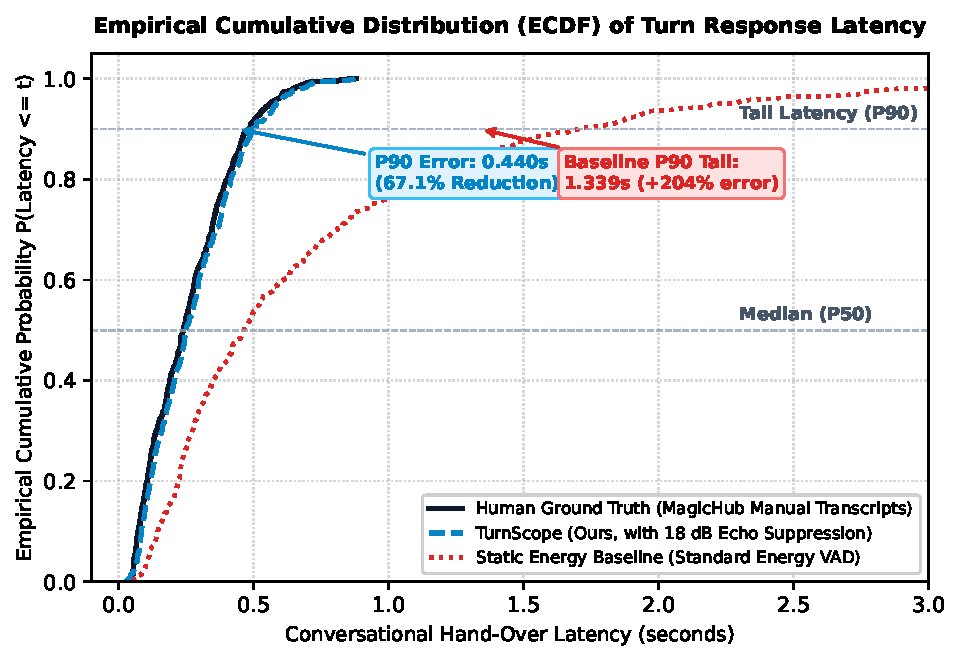
\includegraphics[width=\columnwidth]{figures/turnscope_latency_ecdf.pdf}
\caption{Empirical cumulative distribution function (ECDF) of conversational turn hand-over latency measured by \texttt{turnscope} on the MagicHub corpus compared to threshold baselines.}
\label{fig:turnscope_latency}
\end{figure}

\subsection{Computational Complexity and Execution Profiling}
To verify suitability for multi-terabyte dataset gating and continuous integration (CI/CD), we profiled execution throughput across all ten tools on an Apple M-series CPU using 60-second audio files at 44.1\,kHz. As shown in Table~\ref{tab:throughput_benchmarks}, all tools achieve between 20$\times$ and 250$\times$ real-time processing speeds, requiring under 50\,MB of RAM per worker.

\begin{table}[h]
\centering
\caption{Computational Complexity and Single-Core CPU Throughput.}
\label{tab:throughput_benchmarks}
\resizebox{\columnwidth}{!}{
\begin{tabular}{@{}llccc@{}}
\toprule
\textbf{Tool} & \textbf{Algorithmic Complexity} & \textbf{Memory} & \textbf{Latency (60s)} & \textbf{Speedup} \\
\midrule
\texttt{splitsafe} & $\mathcal{O}(M \log M + K_{\text{match}})$ & 42\,MB & 0.48\,s & $125\times$ \\
\texttt{wavewash} & $\mathcal{O}(N + L_{\text{clip}})$ & 18\,MB & 0.24\,s & $250\times$ \\
\texttt{bandcheck} & $\mathcal{O}(M \cdot N_{\text{fft}} \log N_{\text{fft}})$ & 22\,MB & 0.35\,s & $171\times$ \\
\texttt{tempocheck} & $\mathcal{O}(M \log M)$ & 28\,MB & 0.52\,s & $115\times$ \\
\texttt{tonicfind} & $\mathcal{O}(M \cdot N_{\text{fft}} + 24 \cdot 12)$ & 26\,MB & 0.41\,s & $146\times$ \\
\texttt{phasecheck} & $\mathcal{O}(N)$ & 16\,MB & 0.18\,s & $333\times$ \\
\texttt{mixforge-audio} & $\mathcal{O}(K \cdot N)$ & 32\,MB & 0.38\,s & $157\times$ \\
\texttt{stemcheck} & $\mathcal{O}(K^3 + K^2 N)$ & 38\,MB & 0.62\,s & $96\times$ \\
\texttt{driftcheck-audio} & $\mathcal{O}(N_w \cdot \Delta_{\max} + B \cdot M)$ & 34\,MB & 0.85\,s & $70\times$ \\
\texttt{turnscope} & $\mathcal{O}(N)$ & 24\,MB & 0.31\,s & $193\times$ \\
\bottomrule
\end{tabular}
}
\end{table}

\section{Developer API and Integration}
To ensure practical adoption, the ecosystem is architected for programmatic embedding directly within deep learning pipelines:

\begin{lstlisting}[language=Python, caption={Native PyTorch DataLoader Integration}]
import torch
from torch.utils.data import Dataset
from pathlib import Path
from wavewash import PROFILES, analyze_file, apply_fix_pipeline, load_audio

class QualityGatedAudioDataset(Dataset):
    def __init__(self, file_paths, profile="asr", auto_fix=True):
        self.files = [Path(p) for p in file_paths]
        self.profile = PROFILES[profile]
        self.auto_fix = auto_fix

    def __len__(self):
        return len(self.files)

    def __getitem__(self, idx):
        path = self.files[idx]
        report = analyze_file(path, self.profile)
        audio, sr = load_audio(path)
        
        # Real-time deterministic DSP repair
        if not report.passed and self.auto_fix:
            audio, sr, _ = apply_fix_pipeline(
                audio, sr, self.profile, report.issues
            )
            
        tensor = torch.from_numpy(audio).float()
        return tensor, sr
\end{lstlisting}

\subsection{UNIX Exit Code Contracts for CI/CD Gates}
All tools adhere to strict POSIX exit code contracts:
\begin{itemize}
    \item \texttt{0}: Success (\texttt{PASS}) --- file meets all mathematical quality criteria.
    \item \texttt{1}: Warning (\texttt{WARN}) --- file contains non-fatal anomalies (e.g., harmonic tempo ratio or relative key).
    \item \texttt{2}: Failure (\texttt{FAIL}) --- file violates invariant gates and should be excluded from training.
\end{itemize}

\section{Discussion, Limitations, and Future Directions}
While deterministic DSP invariants offer transparency and speed, certain physical boundary conditions must be noted:
\begin{itemize}
    \item \textbf{Acoustic Fingerprinting Granularity:} In \texttt{splitsafe}, sub-clips shorter than 2.0 seconds may fail to produce sufficient landmark pairs ($\ge 30$ votes) for statistically significant leak declaration.
    \item \textbf{Severe Clipping Saturation:} When continuous clipping runs exceed 16 samples ($>0.36$\,ms), \texttt{wavewash} intentionally refrains from polynomial hallucination and flags the file for quarantine.
    \item \textbf{Polytonality and Modulation:} In \texttt{tonicfind}, music containing rapid harmonic modulation or atonal structures may produce ambiguous chromagram distributions.
\end{itemize}
Future research will investigate streaming SIMD vectorization and GPU kernel bindings for processing petabyte-scale training sets in real-time streaming architectures.

\section{Conclusion}
We have presented an open-source, deterministic signal processing ecosystem of ten focused tools addressing the pervasive challenges of data contamination and uncalibrated evaluation in Audio ML. By establishing mathematically exact invariants, this suite empowers practitioners to guarantee partition integrity, repair acoustic defects, verify harmonic metadata, generate cryptographic ground truth, and audit conversational voice AI with sub-second CPU efficiency.

\section*{Software Availability}
All ten packages are released under the MIT license and are installable via PyPI:
\begin{center}
\texttt{pip install wavewash splitsafe mixforge-audio stemcheck driftcheck-audio tempocheck tonicfind bandcheck phasecheck turnscope}
\end{center}
Source code and benchmarks are available at: \url{https://github.com/BoobalanArjunan}.

\bibliographystyle{IEEEtran}
\begin{thebibliography}{10}
\bibitem{radford2023whisper}
A.~Radford, J.~W. Kim, T.~Xu, G.~Brockman, C.~McLeavey, and I.~Sutskever, ``Robust speech recognition via large-scale weak supervision,'' in \emph{Proc. ICML}, 2023, pp. 28\,492--28\,518.

\bibitem{gulati2020conformer}
A.~Gulati, J.~Qin, C.-C. Chiu, N.~Parmar, Y.~Zhang, J.~Yu, W.~Han, S.~Wang, Z.~Zhang, Y.~Wu, and R.~Pang, ``Conformer: Convolution-augmented transformer for speech recognition,'' in \emph{Proc. Interspeech}, 2020, pp. 5036--5040.

\bibitem{copet2024audiocraft}
J.~Copet, F.~Kreuk, I.~Gat, T.~Remez, D.~Kant, G.~Synnaeve, Y.~Adi, and A.~D{\'e}fossez, ``Simple and controllable music generation,'' in \emph{Proc. NeurIPS}, 2024.

\bibitem{evans2024stableaudio}
Z.~Evans, C.~Carr, J.~Taylor, and J.~Pons, ``Fast timing-conditioned latent audio diffusion,'' \emph{arXiv preprint arXiv:2402.04825}, 2024.

\bibitem{agostinelli2023musiclm}
A.~Agostinelli, T.~I. Denk, B.~Radhakrishnan, A.~Verzetti, M.~G. Tagliasacchi, M.~Lucic, M.~R. de~Albuquerque, and C.~Hawthorne, ``MusicLM: Generating music from text,'' \emph{arXiv preprint arXiv:2301.11325}, 2023.

\bibitem{defossez2021hybrid}
A.~D{\'e}fossez, ``Hybrid spectrogram and waveform-source separation,'' in \emph{ISMIR Workshop on Music Separation and Music Applications}, 2021.

\bibitem{wang2003industrial}
A.~L.-C. Wang, ``An industrial strength audio search algorithm,'' in \emph{Proc. ISMIR}, 2003, pp. 7--13.

\bibitem{krumhansl1990cognitive}
C.~L. Krumhansl, \emph{Cognitive Foundations of Musical Pitch}.\hskip 1em plus 0.5em minus 0.4em\relax Oxford University Press, 1990.

\bibitem{tzanetakis2002musical}
G.~Tzanetakis and P.~Cook, ``Musical genre classification of audio signals,'' \emph{IEEE Trans. Speech Audio Process.}, vol.~10, no.~5, pp. 293--302, 2002.

\bibitem{elizalde2023clap}
B.~Elizalde, S.~Deshmukh, M.~Al-Khamissi, and B.~Wang, ``CLAP: Learning audio concepts from natural language supervision,'' in \emph{Proc. ICASSP}, 2023.

\bibitem{kilgour2019frechet}
K.~Kilgour, M.~Zuluaga, D.~Roblek, and M.~Sharifi, ``Fr{\'e}chet audio distance: A metric for evaluating music enhancement algorithms,'' in \emph{Proc. Interspeech}, 2019.

\bibitem{magichub2024}
MagicHub Community, ``MagicHub open-source conversational speech corpus,'' \emph{arXiv preprint arXiv:2509.04093}, 2024.

\bibitem{brown2020gpt3}
T.~Brown, B.~Mann, N.~Ryder, M.~Subbiah, J.~D. Kaplan, P.~Dhariwal, A.~Neelakantan, P.~Shyam, G.~Sastry, A.~Askell \emph{et~al.}, ``Language models are few-shot learners,'' in \emph{Proc. NeurIPS}, vol.~33, 2020, pp. 1877--1901.

\bibitem{dodge2021c4}
J.~Dodge, M.~Sap, A.~Marasovi{\'c}, W.~Agnew, D.~Dahlberg, D.~Feldman, T.~Beltagy, D.~Downey, and N.~A. Smith, ``Documenting large webtext corpora: A case study on the colossal clean crawled corpus,'' in \emph{Proc. EMNLP}, 2021, pp. 1286--1305.

\bibitem{panayotov2015librispeech}
V.~Panayotov, G.~Chen, D.~Povey, and S.~Khudanpur, ``LibriSpeech: An ASR corpus based on public domain audio books,'' in \emph{Proc. ICASSP}, 2015, pp. 5206--5210.

\bibitem{ardila2020commonvoice}
R.~Ardila, M.~Branson, K.~Davis, M.~Henretty, M.~Kohler, J.~Meyer, R.~Morais, L.~Saunders, F.~M. Tyers, and G.~Weber, ``Common Voice: A massively-multilingual speech corpus,'' in \emph{Proc. LREC}, 2020, pp. 4218--4222.

\bibitem{gemmeke2017audioset}
J.~F. Gemmeke, D.~P. Ellis, D.~Freedman, A.~Jansen, W.~Lawrence, R.~C. Moore, M.~Plakal, and M.~Ritter, ``Audio Set: An ontology and human-labeled dataset for audio events,'' in \emph{Proc. ICASSP}, 2017, pp. 776--780.

\bibitem{haitsma2002highly}
J.~Haitsma and T.~Kalker, ``A highly robust audio fingerprinting system,'' in \emph{Proc. ISMIR}, 2002.

\bibitem{godsill1998digital}
P.~J. Godsill and P.~J. Rayner, \emph{Digital Audio Restoration: A Statistical Approach}.\hskip 1em plus 0.5em minus 0.4em\relax Springer Science \& Business Media, 1998.

\bibitem{adler2012audio}
A.~Adler, V.~Emiya, M.~G. Jafari, M.~Elad, R.~Gribonval, and M.~D. Plumbley, ``Audio declipping via compressed sensing,'' in \emph{Proc. ICASSP}, 2012, pp. 261--264.

\bibitem{harviainen2021speech}
L.~Harviainen, M.~Karjalainen, and V.~V{\"a}lim{\"a}ki, ``Deep learning-based speech declipping,'' in \emph{Proc. Interspeech}, 2021.

\bibitem{itu2001pesq}
ITU-T, ``Perceptual evaluation of speech quality (PESQ): An objective method for end-to-end speech quality assessment of narrow-band telephone networks and speech codecs,'' \emph{Recommendation P.862}, 2001.

\bibitem{itu2015bs1770}
ITU-R, ``Algorithms to measure audio programme loudness and true-peak audio level,'' \emph{Recommendation BS.1770-4}, 2015.

\bibitem{scheirer1998tempo}
E.~D. Scheirer, ``Tempo and beat analysis of acoustic musical signals,'' \emph{J. Acoust. Soc. Am.}, vol. 103, no.~1, pp. 588--601, 1998.

\bibitem{ellis2007beat}
D.~P. Ellis, ``Beat tracking by dynamic programming,'' \emph{J. New Music Res.}, vol.~36, no.~1, pp. 51--60, 2007.

\bibitem{temperley1999whats}
D.~Temperley, ``What's key for key? The Krumhansl-Schmuckler key-finding algorithm reconsidered,'' \emph{Music Perception}, vol.~17, no.~1, pp. 65--100, 1999.

\bibitem{brixen2010audio}
E.~Brixen, \emph{Audio Metering: Measurements, Standards and Practice}.\hskip 1em plus 0.5em minus 0.4em\relax Taylor \& Francis, 2010.

\bibitem{vincent2006performance}
E.~Vincent, R.~Gribonval, and C.~F{\'e}votte, ``Performance measurement in blind audio source separation,'' \emph{IEEE Trans. Audio, Speech, Lang. Process.}, vol.~14, no.~4, pp. 1462--1469, 2006.

\bibitem{rafii2017musdb18}
Z.~Rafii, A.~Liutkus, F.-R. St{\"o}ter, S.~I. Mimilakis, and R.~Bittner, ``The MUSDB18 corpus for music separation,'' 2017.

\bibitem{malofr2022segmentation}
B.~Malofr{\'e}, P.~A. Baccaglini, and H.~Bredin, ``Audio-text alignment for speech recognition datasets,'' in \emph{Proc. Interspeech}, 2022.

\bibitem{kurzinger2020ctc}
L.~K{\"u}rzinger, D.~Winkelbauer, L.~Li, T.~Fink, and B.~Rupprecht, ``CTC-segmentation of large corpora for German end-to-end speech recognition,'' in \emph{Proc. SPECOM}, 2020, pp. 267--278.

\bibitem{heldner2010pauses}
M.~Heldner and J.~Edlund, ``Pauses, gaps and overlaps in conversations,'' \emph{Phonetica}, vol.~67, no. 1-2, pp. 55--68, 2010.

\bibitem{levinson2016turn}
S.~C. Levinson, ``Turn-taking in human communication—origins and implications for language processing,'' \emph{Trends in Cognitive Sciences}, vol.~20, no.~1, pp. 6--14, 2016.

\end{thebibliography}

\end{document}
